\documentclass{entcs} 
\usepackage{CSC8498macro}
\usepackage{graphicx}
\graphicspath{{./Images/}}

%% This document describes the formatting instructions for the CSC8498 final report.

\makeatletter

\def\lastname{Boulderstone}
\begin{document}

\begin{frontmatter}
\title{Rollback Netcode, Implmentation and Adoption}
\author{Edward Boulderstone}
  \address{School of Computing Science, Newcastle University, UK} 
\thanks[nigellemail]{Email:
    \href{mailto:E.Boulderstone@ncl..ac.uk} {\texttt{\normalshape
        E.Boulderstone@ncl..ac.uk}}}

			
				
\begin{abstract} 
Rollback netcode is a peer to peer networking soultion. It had potential to improve online experiences by minimizing the effects of latency over traditional delay based . However the implementation of rollback netcode in the fighting game industry has been slow and difficult. This project aims to understand  understand how the industry has had difficulty implementing rollback, and find any optimizations that can be made to existing public rollback netcode understanding.
\end{abstract}

\begin{keyword}
rollback, netcode, peer to peer, fighting games, networking, industry.
\end{keyword}
\end{frontmatter}

\section{Introduction}\label{sec: introduction}
The goal of networking in video games is to allow people from all over the world to play with each other. However fans of fighting games have historically (Before the pandemic) gone out of their way to organise local tournaments with most major tournaments before the pandemic taking place off-line\cite{FGCMajors}. This trend started because of the when fighting games were played in arcades in the mid 1990's,\cite{FirstUSTournament} and continued until the start of the pandemic, in part because fighting games rely on consistent timing and a low latency environment \cite{DelayVsRollback}, \cite{BadNetcode}. The existing networking solutions at the time simply did not provide this environment for competitive play\cite{FGCAsEsport}. However the spread of the corona virus in the mid 2020's fighting games found themselves having to fall back onto these "lower quality" online platforms. Games which did not have well optimized netcode found themselves on the back foot, with reduced attention \cite{SmashTournamentsInThePandemic}, and games with well written netcode found their success  \cite{GuiltyGearStriveInThePandemic}.

\subsection{Delay Based Netcode}
The first solution to online play for fighting games was a peer to peer system known as delay based netcode. Peer to peer netcode is important for fighting games because of the aforementioned need for low latency. Because most fighting games are between two players \cite{FightingGameDefine}, introducing a server will increase the ping between the two players, as the information has to travel to a seperate location, before being sent to the opposing player. 


Delay based netcode works by keeping two players in lockstep, meaning that each player's simulation of the game are paused whilst waiting for the input from the other player\cite{DelayBasedNetcode}. This system works well when latency is not a major factor, for example, in a turn based game, where the inputs are spread apart by seconds, a pause of half a second may go unnoticed. To address packets taking time to travel between two remote players, a number of input delay frames are added. Input delay frames delay the game state by a number of frames, and allow the local inputs to be sent ahead of time. So if the remote input arrives before the input delay frames are finished, there is no pause \ref{fig:DelayBasedNetcodeRepresentation}.

\begin{figure}[h]
\centering
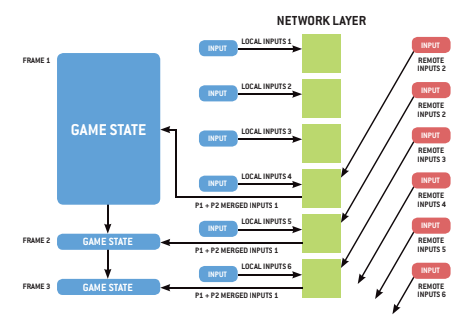
\includegraphics{DelayBasedNetcodeRepresentation}
\caption{Delay based netcode \cite{GGPODocumentation}}
\label{fig:DelayBasedNetcodeRepresentation}
\end{figure}

\subsection{Rollback Netcode}
Rollback netcode was developed in 2006 as a solution to the problems with delay based netcode. \cite{RollbackDevelopment}. It works on top of existing delay based netcode by adding rollback frames, predicting the remote users inputs. When the remote user's input arrives if it matches with the predicted input, nothing happens, however if there's a discrepancy the game will "rollback", to the point of the discrepancy and re-simulate the game state back to the real time frame \ref{fig:RollbackNetcodeRepresentation}.

\begin{figure}[h]
\centering
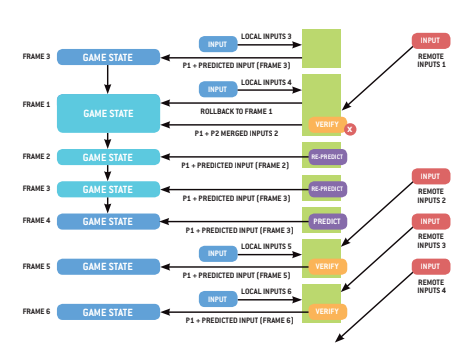
\includegraphics{RollbackNetcodeRepresentation}
\caption{Rollback netcode \cite{GGPODocumentation}}
\label{fig:RollbackNetcodeRepresentation}
\end{figure}
\newpage
\subsection{Difficulties in industry}
In today's fighting game market, many games have rollback \cite{GamesWithRollback}.However there are still notable exceptions such as:
\begin{itemize}
\item Super Smash Bros. Ultimate\cite{SSBU}
\item Granblue Fantasy Versus\cite{GBFV}
\item Under Night In-Birth\cite{UNI}
\item Samurai Shodown\cite{SamSho}
\item Soulcalibur VI\cite{SVI}
\item Dead or Alive 6\cite{DOA6}
\item EA Sports UFC 4\cite{UFC4}
\item Dragon Ball FighterZ\cite{DBFZ}
\end{itemize}

Other fighting games have had difficulty in implementing rollback, such as Street fighter V and Mortal Kombat X.
These difficulties with implementing and developing rollback are the basis of the motivation of this paper.

\subsection{Aim}
To investigate rollback netcode, it's usage in industry and any short comings of existing public rollback netcode infrastructure
\subsection{Objectives}
\begin{itemize}
\item Understand rollback netcode and the effects on the games it's implemented in.
\item Create a visualization for the differences between rollback and delay based netcode.
\item Research the difficulties of implementing rollback in existing games.
\item Explore optimizations for the existing public rollback structure.
\item Investigate further uses of rollback netcode, in the wider video game industry.
\end{itemize}
\newpage
\section{What you did and how}

\section{Background}
\subsection{Delay based netcode}
\subsection{Rollback netcode}
\subsection{Difficulties in Implmentation}
- separate gameplay from rendering
- serializable game state
- particle simulation 
- object lifetime 
- sound fx
- animation system
- UI
- desync detection
\subsubsection{One sided Rollback}
\subsubsection{Street Fighter V}
\subsubsection{Mortal Kombat X}
\subsection{Third party Rollback}

\section{Effects of Rollback on Game Design}
\subsection{8 Frames}
\subsection{Audio Design}
\subsection{Visual Design}


\section{Improvements for Rollback}
\subsection{Prediction Quality}
\subsection{Packet Contents Optimization}
\subsection{Input Locking}

\section{Rollback Visualization tool}
\subsection{Design}

\section{Wider use case of rollback netcode}
Rollback ideas that only apply to fighting games? (Visual teleportation?, Expensive to implement?, ) 
 RTS (Including sports games)

\section{Evaluation}

This section might alternatively be called “Experimental results”.  It describes how you assessed your project and what you found out. Where you give results in tables or graphs, remember to highlight in the text the key points that the data shows and, if possible, try to explain why you got any unexpected results.

\section{Conclusions and further work}

In this section you summarise what you did and discovered and (importantly) what else you would have done (or done differently) if you had the chance. It is a chance to reflect on your success.

\begin{thebibliography}{25}

\bibitem{GGPODocumentation} {\texttt https://drive.google.com/file/d/1nRa3cRBQmKj0-SEyrT\_1VNOkPOJWNhVI/view} or 
{\texttt https://web.archive.org/web/20220101162600/https://drive.google.com/file/d/1nRa3cRBQmKj0-SEyrT\_1VNOkPOJWNhVI/view} 
Tony C., GGPO Game Developer Magazine's article. 2012. (Visited 25/05/2022)

\bibitem{FGCMajors} {\texttt https://liquipedia.net/fighters/Tier\_1\_Tournaments} or 
{\texttt https://web.archive.org/web/20210121113554/https://liquipedia.net/fighters/Tier\_1\_Tournaments} 
Liquidpedia list of major fighting game tournaments. (Visited 25/05/2022)

\bibitem{FirstUSTournament} {\texttt https://www.usgamer.net/articles/the-oral-history-of-evo} or 
{\texttt https://web.archive.org/web/20220321000753/https://www.usgamer.net/articles/the-oral-history-of-evo} 
John L., The Oral History of EVO: The Story of the World's Largest Fighting Game Tournament (Visited 25/05/2022)

\bibitem{FGCAsEsport} {\texttt https://esportsinsider.com/2021/10/can-fighting-games-become-a-mainstream-esport/} or 
{\texttt https://web.archive.org/web/20220516060805/https://esportsinsider.com/2021/10/can-fighting-games-become-a-mainstream-esport/} 
Elizbar R., Can fighting games become a mainstream esport without abandoning grassroots?. (Visited 26/02/2022) 

\bibitem{SmashTournamentsInThePandemic} {\texttt https://www.ssbwiki.com/COVID-19\_pandemic\_and\_its\_impact\_on\_competitive\_Smash} or {\texttt https://web.archive.org/web/20220516020551/https://www.ssbwiki.com/COVID-19\_pandemic\_and\_its\_impact\_on\_competitive\_Smash} List of smash tournaments affected by the pandemic. (Visited 26/02/2022) 

\bibitem{GuiltyGearStriveInThePandemic} {\texttt https://techraptor.net/gaming/opinions/guilty-gear-strive-changed-fighting-games-rollback-netcode} or {\texttt https://web.archive.org/web/20210713144527/https://techraptor.net/gaming/opinions/guilty-gear-strive-changed-fighting-games-rollback-netcode} Davi B. Guilty Gear Strive Might Have Changed Fighting Games Forever. (Visited 26/02/2022)

\bibitem{DelayVsRollback} {\texttt https://arstechnica.com/gaming/2019/10/explaining-how-fighting-games-use-delay-based-and-rollback-netcode/} or {\texttt https://web.archive.org/web/20220425211823/https://arstechnica.com/gaming/2019/10/explaining-how-fighting-games-use-delay-based-and-rollback-netcode/} Ricky P. Explaining how fighting games use delay-based and rollback netcode. (Visted 26/05/2022)

\bibitem{BadNetcode} {\texttt https://www.polygon.com/2020/3/25/21192522/netcode-samurai-showdown-fighting-games-rollback-delay} or {\texttt https://web.archive.org/web/20220401231646/https://www.polygon.com/2020/3/25/21192522/netcode-samurai-showdown-fighting-games-rollback-delay} David C. Bad netcode is killing many of your favorite fighting
games. (Visted 26/05/2022)

\bibitem{RollbackDevelopment} {\texttt https://gamasutra.com/view/news/34050/Interview\_How\_A\_Fighting\_Game\_Fan\_Solved\_Internet\_Latency

\_Issues.php} or {\texttt https://web.archive.org/web/20220325062609/https://gamasutra.com/view/news/34050/Interview\_How\_A\_Fighting\_Game\_Fan\_Solved\_Internet\_Latency\_Issues.php} Kyle O. Interview: How A Fighting Game Fan Solved Internet Latency Issues. (Visted 26/05/2022)

\bibitem{FightingGameDefine} {\texttt https://archive.org/details/nextgen-issue-015/page/n33/mode/2up} "The Next Generation 1996 Lexicon A to Z: Fighting Game". (Visited 26/05/2022)

\bibitem{DelayBasedNetcode} {\texttt https://www.gamasutra.com/view/feature/3094/1500\_archers\_on\_a\_288\_network\_.php} or {https://web.archive.org/web/20220506231117/https://www.gamasutra.com/view/feature/3094/1500\_archers\_on\_a\_288\_network\_.php} Mark T. 1500 Archers on a 28.8: Network Programming in Age of Empires and Beyond. (Visted 26/05/2022)

\bibitem{FightingGameNetworking} {\texttt https://web.archive.org/web/20210228051849/https://mauve.mizuumi.net/2012/07/05/understanding-fighting-game-networking.html} Mauve M. Understanding Fighting Game Networking. (Visted 26/05/2022)

\bibitem{GamesWithRollback} {\texttt https://attackofthefanboy.com/guides/rollback-netcode-games-list/} or {\texttt https://web.archive.org/web/20211122034207/https://attackofthefanboy.com/guides/rollback-netcode-games-list/} Andron S. Rollback Netcode Games List (March 2022). (Visted 26/05/2022)

\bibitem{SSBU} {\texttt https://en.wikipedia.org/wiki/Super\_Smash\_Bros.\_Ultimate} or {\texttt https://web.archive.org/web/20220519200835/https://en.wikipedia.org/wiki/Super\_Smash\_Bros.\_Ultimate} Super Smash Bros. Ultimate. (Visited 26/05/2022)

\bibitem{GBFV} {\texttt https://en.wikipedia.org/wiki/Granblue\_Fantasy\_Versus} or {\texttt https://web.archive.org/web/20220512125807/https://en.wikipedia.org/wiki/Granblue\_Fantasy\_Versus} Grandblue Fantasy Versus (Visited 26/05/2022)

\bibitem{UNI} {\texttt https://en.wikipedia.org/wiki/Under\_Night\_In-Birth} or {\texttt https://web.archive.org/web/20220516020108/https://en.wikipedia.org/wiki/Under\_Night\_In-Birth} Under Night In-birth (Visited 26/05/2022)

\bibitem{SamSho} {\texttt https://en.wikipedia.org/wiki/Samurai\_Shodown\_(2019\_video\_game)} or {\texttt https://web.archive.org/web/20220504020927/https://en.wikipedia.org/wiki/Samurai\_Shodown\_(2019\_video\_game)} Samurai Shodown (Visited 26/05/2022)

\bibitem{SVI} {\texttt https://en.wikipedia.org/wiki/Soulcalibur\_VI} or {\texttt https://web.archive.org/web/20220421074040/https://en.wikipedia.org/wiki/Soulcalibur\_VI} Soulcalibur VI (Visited 26/05/2022)

\bibitem{DOA6} {\texttt https://en.wikipedia.org/wiki/Dead\_or\_Alive\_6} or {\texttt https://web.archive.org/web/20220130144906/https://en.wikipedia.org/wiki/Dead\_or\_Alive\_6} Dead or Alive 6 (Visited 26/05/2022)

\bibitem{UFC4} {\texttt https://en.wikipedia.org/wiki/EA\_Sports\_UFC\_4} or {\texttt https://web.archive.org/web/20211019192531/https://en.wikipedia.org/wiki/EA\_Sports\_UFC\_4} EA Sports UFC 4 (Visited 26/05/2022)

\bibitem{DBFZ} {\texttt https://en.wikipedia.org/wiki/Dragon\_Ball\_FighterZ} or {\texttt https://web.archive.org/web/20220424200258/https://en.wikipedia.org/wiki/Dragon\_Ball\_FighterZ} Dragon Ball FighterZ (Visited 26/05/2022)

\end{thebibliography}
\end{document}
